\chapter{AMD SEV}

\section{History and Iterations}
\begin{itemize}
    \item \textbf{SEV:} Called vanilla SEV or SCV, it was introduced with AMD EPYC NAPLES (7001) ~2016 and provide VM memory encryption (guest isolation from one to one another)
    \item \textbf{SEV-ES:} Introduced with AMD EPYC ROME (7002) ~2019, it provides encryption state and the protection for register stats
    \item \textbf{SEV-SNP:} Introduced with AMD EPYC MILAN (7003) ~2021, it provides secure nested paging and a strongest memory integrity protection
\end{itemize}

All the three version are based on AMD-V virtualization extension and AMD-PSP introduced back in 2013.

\section{SEV: Architecture}

SEV, briefly, provide isolation between one guest and another. \\
It assigne an \textbf{ACID} (Address Space IDentifier) to each guest for tags all the memory accesses of a guest. (It's also put it to the TLB and cache as extra tag). \\
Each guest virtual machine (VM) in the Secure Encrypted Virtualization (SEV) architecture is assigned its own unique encryption key: Virtual Machine Encryption Key (VEK). 
The encryption of guest memory is performed by the Unified Memory Controller (UMC) using AES-128-XEX or AES-256-XTS. The VEKs are both generated and securely stored within the AMD Secure Processor (PSP). 
The VEK remains valid for the entire lifetime of the guest VM, or if the VM is migrated to a different platform, a new VEK is generated in the remote platform. This process guarantees the gust VM memory confidentiality but not the integrity.

\begin{figure}[h]
    \centering
    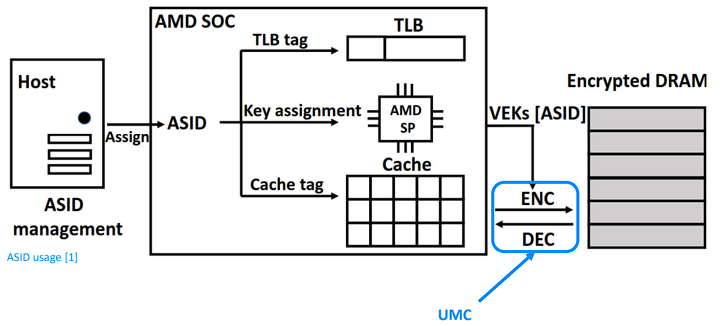
\includegraphics[width=0.8\textwidth]{img/sev-arch.png}
    \caption{SEV Architecture Overview}
    \label{fig:sev_architecture}
\end{figure}

\section{SEV-ES: Architecture}

SEV-ES extends the capabilities of the original SEV architecture by introducing protections for register states, 
ensuring their security even when a virtual machine (VM) stops running. 
The threat model remains consistent with the original SEV design, assuming a benign but vulnerable hypervisor. 
In the earlier SEV implementation, when a VM halts, its register states are stored in the Virtual Machine Control Block (VMCB), which resides in the hypervisor's memory. 
This arrangement leaves the register states susceptible to unauthorized extraction or tampering. SEV-ES addresses this vulnerability by safeguarding the contents of the VMCB. 
The VMCB contains critical information and data required to properly resume the guest VM after it has been paused, making its protection essential for maintaining the security and integrity of virtualized environments. \bigskip

So, In SEV-ES the VMCB (Virtual Machine Control Block) is divided in VMSA and VMCA:
\begin{itemize}
    \item \textbf{VMSA:} is stored in the encrypted memory area (the hypervisor can't access it)
    \item \textbf{VMCA:} is unencrypted as it's needed to the hypervisor for managing the guest VM
\end{itemize}

SEV-ES also introduce the \textbf{GHCB} (Guest-Hypervisor Communication Block) to share date between the guest and the hypervisor and it's used for ACPI virtualization.

\subsection{VM Lifecycle Management}

For stop a VM is used the \textbf{VMGEXIT} instruction that save all the register states in the VMSA that is is the encrypted memory area. 
Then Computes the hash of the register states and stores it in a protected memory region for guarantee the integrity of the VM at resume. \bigskip

For resume a VM is used the \textbf{VMRUN} that as first thing check the integrity of the VM by computing the hash of the VMSA's content, compared to the hash to the previous one stored.
Then the VMSA registers content is restored and the VM is resumed. 

The change of a VM from running to stopped is called \textbf{World Switch}.
\begin{figure}[h]
    \centering
    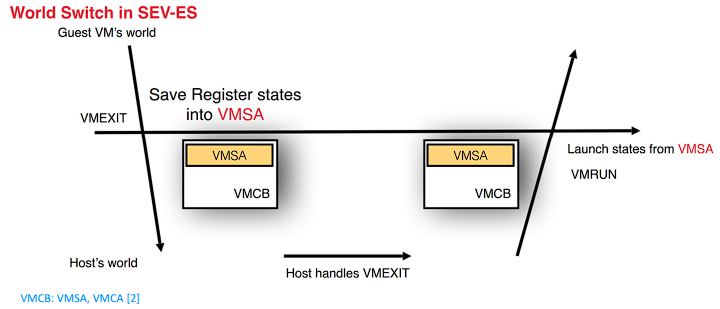
\includegraphics[width=0.8\textwidth]{img/world-switch-es.png}
    \caption{SEV-ES World Switch}
    \label{fig:world_switch_es}
\end{figure}

\section{SEV-SNP: Architecture}
\begin{boxH}
    Change in the Threat Model: Nothing is trusted, apart from AMD hardware and firmware.
\end{boxH}

Some feature are direclty built from SEV-ES and SEV, like the Memory encrypted with inline AES and the register state encrypted and atomically swapped. \bigskip

There are some new feature as the VM memory integrity protection from:
\begin{itemize}
    \item VM memory replacement with old copy
    \item VM memory corruption
    \item Aliasing: assignment of two guest pages to same DRAM page
    \item Remapping: Switch DRAM page mapped to a guest page
\end{itemize}

After that follows the provided protection from cold boot attacks (but does not provides protection from DoS attacks from the hypervisor)

\begin{figure}[h]
    \centering
    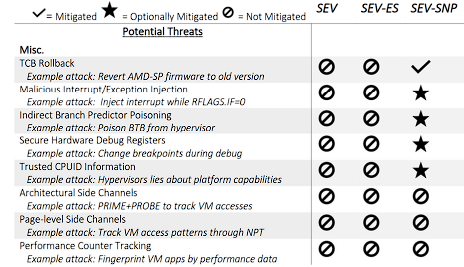
\includegraphics[width=0.8\textwidth]{img/SEV-comp.png}
    \caption{Table of SEV, SEV-ES and SEV-SNP comparison}
    \label{fig:sev_comp}
\end{figure}

\subsection{ Integrity enforcement}

SEV-SNP enforces memory integrity through a specialized data structure known as the Reverse Map Table (\textbf{RMP}). 
This table is created during the system's boot process, with one RMP table allocated per system. Each entry in the RMP corresponds to a \textbf{4KB} block of assignable memory and is indexed by the System Physical Address (\textbf{SPA}).
These entries store crucial information about the ownership of each memory page, along with additional metadata, which collectively determine whether the page is writable. 
Specific restrictions are enforced to ensure memory security: pages allocated for the hypervisor cannot be repurposed as encrypted pages, and pages reserved for AMD firmware are strictly read-only, preventing any unauthorized modifications. 
This robust mechanism helps maintain the integrity and isolation of guest memory in virtualized environments.

\subsubsection{RMP checks}
The Reverse Map Table (RMP) checks ensure that memory operations are properly validated depending on the context and mode of access. \\
The RMP table is checked in the following scenarios: 
    \begin{itemize} 
        \item During writes in all modes. 
        \item During reads initiated by SEV-SNP guests. 
    \end{itemize} 
It is not checked during reads performed in hypervisor (HV) mode, as the memory in this mode is encrypted and deemed secure by design. 


Key terminology for understanding RMP checks includes: 
\begin{itemize} 
    \item \textbf{GPA (Guest Physical Address)}: The memory address as perceived by the guest VM. 
    \item \textbf{GVA (Guest Virtual Address)}: The virtual memory address used within the guest VM. 
    \item \textbf{GR3 (Guest Register 3)}: A register that contains the physical address of the base of the host's page table hierarchy.
    \item \textbf{gGR3}: The guest-specific version of GR3, relevant within the guest's context. 
\end{itemize}

\begin{figure}[h]
    \centering
    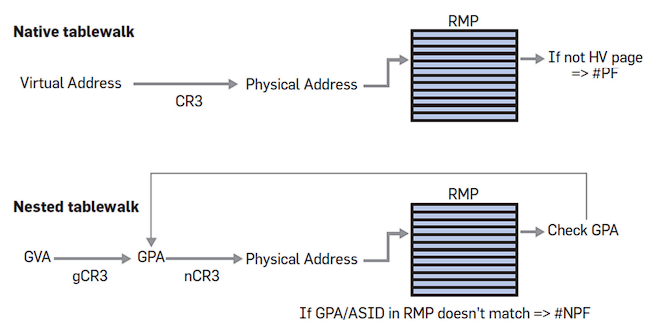
\includegraphics[width=0.8\textwidth]{img/RMP-tablewalk.png}
    \caption{RMP Table Walk}
    \label{fig:rmp_tablewalk}
\end{figure}

\subsection{Page Validation: Page Remapping}

Page validation in SEV-SNP is a critical mechanism designed to protect against memory remapping attacks by ensuring that each Guest Physical Address (\textbf{GPA}) maps to only one valid System Physical Address (\textbf{SPA}) at any given time. 
The process begins with the hypervisor assigning a page to the guest using the RMPUPDATE command, which creates a new entry in the Reverse Map Table (RMP). 
Initially, the page is set to an invalid state, rendering it unusable by either the guest or the hypervisor. 
To finalize the assignment, the guest invokes the PVALIDATE operation to accept and validate the page. (Guest validate the GPA only once)

\subsection{SEV-SNP: Attestation}

SNP offers launch and runnign attestation, but we only see the launch attestation. \\
The measurements for the launch attestation of the guest and the platform are done by the PSP that will collect all the measurements and create the attestation report, 
that is verified by the guest owner by compare the attestation report data against the golden values.

\begin{figure}[h]
    \centering
    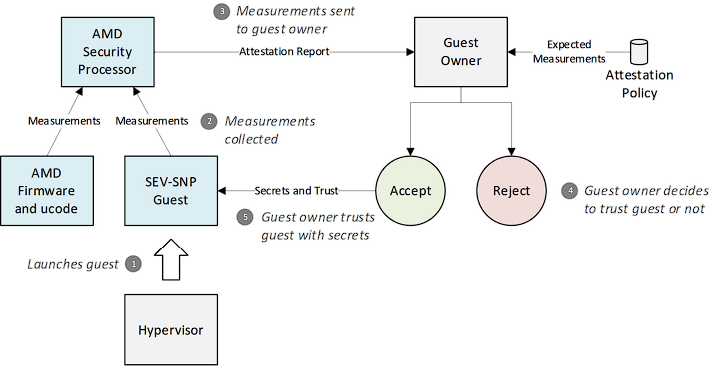
\includegraphics[width=0.8\textwidth]{img/SNP-Attestation-schema.png}
    \caption{SEV-SNP Attestation Schema}
    \label{fig:snp_attestation}
\end{figure}

\subsubsection{Attestation Component}

\begin{multicols}{2}
    \begin{itemize}[itemsep=0pt]
        \item \textbf{Platform measurements}
        \begin{itemize}[itemsep=0pt]
            \item Platform versioning
            \item Platform runtime configuration
            \item Chip Identification
        \end{itemize}
        \item \textbf{Guest measurements}
        \begin{itemize}[itemsep=0pt]
            \item Owner identification
            \item Guest image identification
            \item Initialization of image measurement
            \item SNP guest policies
            \item Migration agents
        \end{itemize}
        \item \textbf{Subsequent actions:}
        \begin{itemize}[itemsep=0pt]
            \item Check the authenticity of the report
            \item Retrieval of the attestation report
            \item Binding of the guest credentials to the report
        \end{itemize}
    \end{itemize}
\end{multicols}

\subsubsection{Attestation guest measurement}

$$LD = hash( LD || Page || Metadata)$$

The guest measurement is done by 3 main commands: \textit{Launch\_start}, \textit{Launch\_update} and \textit{Launch\_finish}. After the \textit{Launch\_finish} the attestation report is produced 
(with the guest owner that have accept or reject the attestation). \\
During the update... \textbf{\textit{Impossibile capire oltre, audio registrato male}} \bigskip

\begin{figure}[h]
    \centering
    \begin{minipage}{0.45\textwidth}
        \centering
        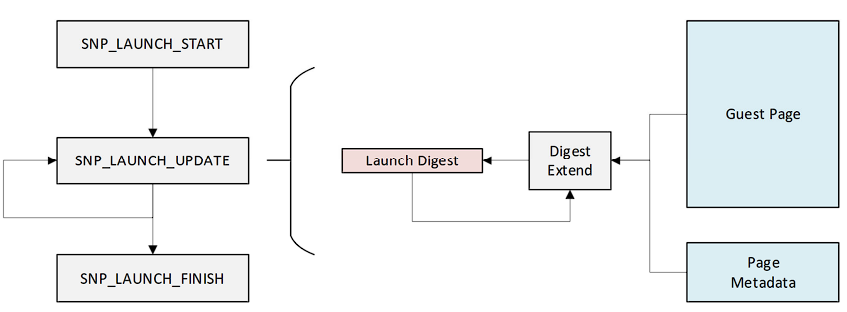
\includegraphics[width=\textwidth]{img/snp-update.png}
        \caption{SNP\_LAUNCH\_UPDATE}
        \label{fig:snp_update}
    \end{minipage}
    \hfill
    \begin{minipage}{0.45\textwidth}
        \centering
        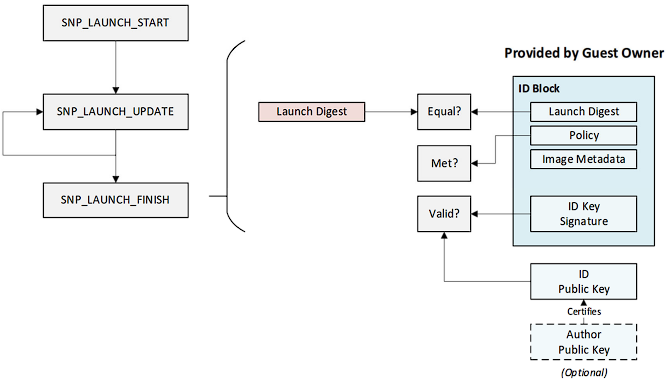
\includegraphics[width=\textwidth]{img/snp-finish.png}
        \caption{SNP\_LAUNCH\_FINISH}
        \label{fig:snp_finish}
    \end{minipage}
\end{figure}


\subsection{Att. Report Authenticity}

The authenticity of the attestation report in the SEV-SNP architecture is ensured through the use of the Versioned Chip Endorsement Key (VCEK), and a new one is derived for each TCB SVN bump. \\

The VCEK is derived from a mix of the TCB versioning and the Chip Unique Secret that is embedded in fuses in the PSP, and then signed by the AMD certificate chain (\textbf{KDS}). 
To be more precise, VCEK is certificate by the AMD SEC VA, that at the same time is certificate by the AMD Root CA. \\
textbf{\textit{Impossibile capire oltre, audio registrato male}} 
\begin{figure}[h]
    \centering
    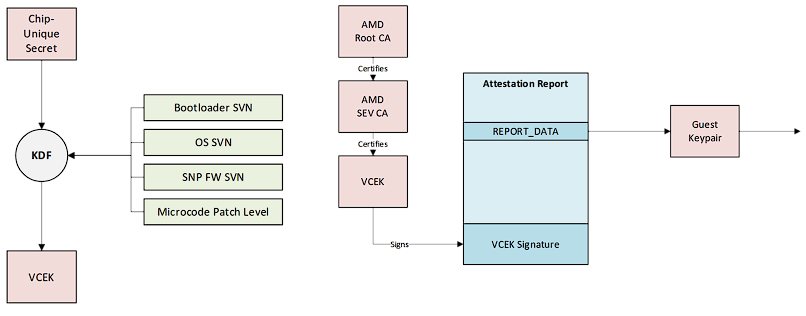
\includegraphics[width=0.8\textwidth]{img/snp-attestation-authenticity.png}
    \caption{SEV-SNP Attestation Report Authenticity}
    \label{fig:snp_attestation_authenticity}
\end{figure}

\section{WeSee: Ahoi Attacks on SEV-SNP}

\subsection{Overview}
The WeSee attack, targets the AMD SEV-SNP architecture by exploiting vulnerabilities related to Virtualization Exception (\#VC) interrupts. These interrupts are maliciously injected by the hypervisor to compromise the guest virtual machine's (VM) integrity.

\subsection{Attack Method}
The attack method revolves around the hypervisor's ability to inject \#VC interrupts into the guest VM. The key mechanism behind the attack is as follows:
\begin{itemize}
    \item The injected interrupts alter the VM's control flow, causing the VM to halt and consume the exception.
    \item This interruption of the VM's normal flow is leveraged by attackers to inject arbitrary code, enabling unauthorized actions inside the guest VM.
\end{itemize}

\subsection{Impact}
The impact of the WeSee attack is significant:
\begin{itemize}
    \item The attack demonstrated the ability to bypass authentication mechanisms in SEV-SNP.
    \item The hypervisor (HV) can exploit SEV-SNP vulnerabilities to gain root shell access inside the guest VM, compromising the VM's security and potentially allowing further attacks.
\end{itemize}

\subsection{Known CVEs and Mitigation}
The vulnerabilities exploited by the WeSee attack are tracked under the following CVE identifiers:
\begin{itemize}
    \item \textbf{CVE-2024-25743}
    \item \textbf{CVE-2024-25744}
\end{itemize}
AMD has addressed these vulnerabilities by releasing a hotfix in the Linux kernel to mitigate the issue.

\subsection{Further Information}
For more details on the attack and its mitigation, visit the official website: \href{https://ahoi-attacks.github.io/wesee/}{WeSee}

